%%%%%%%%%%%%%%%%%%%%%%%%%%%%%%%%%%%%%%%%%%%%%%%%%%%%%%%
% Please note that whilst this template provides a 
% preview of the typeset manuscript for submission, it 
% will not necessarily be the final publication layout.
%
% letterpaper/a4paper: US/UK paper size toggle
% num-refs/alpha-refs: numeric/author-year citation and bibliography toggle


%\documentclass[letterpaper]{oup-contemporary}
\documentclass[a4paper,num-refs]{oup-contemporary}



%%% Journal toggle; only specific options recognised.
%%% (Only "gigascience" and "general" are implemented now. Support for other journals is planned.)%
%\journal{Test}
\jname{Università degli studi Roma Tor Vergata}
\jlogo{}

\usepackage{graphicx}
\usepackage{siunitx}
\usepackage{import}
\usepackage{amsmath}
%\numberwithin{equation}{section}% numera eq come #section.#formula
%

\usepackage{enumitem}
%
\usepackage{amsthm}
\usepackage{stmaryrd}
\usepackage{amssymb}

%
\usepackage{caption}
\usepackage{subcaption}

\usepackage{wasysym}
\usepackage{cancel}
\usepackage{textcomp}
\usepackage{cleveref}
\crefformat{section}{\S#2#1#3} % see manual of cleveref, section 8.2.1
\crefformat{subsection}{\S#2#1#3}
\crefformat{subsubsection}{\S#2#1#3}
\usepackage{lipsum}  
\usepackage{listings}
\definecolor{codegreen}{rgb}{0,0.6,0}
\definecolor{codegray}{rgb}{0.5,0.5,0.5}
\definecolor{codestring}{rgb}{0.4,0.4,0.4}
\definecolor{backcolour}{rgb}{0.96,0.96,0.96}
\definecolor{bbcolour}{rgb}{0.01,0.03,0.35}
\definecolor{indexcolour}{rgb}{0,0.4,0.4}
\lstdefinestyle{mystyle}{
	backgroundcolor=\color{backcolour},   
	commentstyle=\color{codegreen},
	classoffset=1,
	keywordstyle=\color{bbcolour},
	numberstyle=\tiny\color{codegray},
	stringstyle=\color{codestring},
	basicstyle=\ttfamily\small,
	breakatwhitespace=false,  
	breaklines=true,                 
	captionpos=b,                    
	keepspaces=false,                 
	numbers=left,                    
	numbersep=3pt,                  
	showspaces=false,                
	showstringspaces=false,
	showtabs=false,                  
	tabsize=2
}
\lstset{texcl=false, mathescape=true,style=mystyle}
\lstset{emph={%  
		i, j,X,n,Y%
	},emphstyle={\color{indexcolour}}%
}%

\usepackage[euler]{textgreek}


\usepackage{tikz}
\usetikzlibrary{shapes.geometric, arrows}
\tikzstyle{startstop} = [rectangle, rounded corners, minimum width=3cm, minimum height=1cm,text centered, draw=black, fill=backcolour]
\tikzstyle{startstop2} = [rectangle, rounded corners, minimum width=3cm, minimum height=2cm,text centered, draw=black, fill=backcolour]
\tikzstyle{io} = [trapezium, trapezium left angle=70, trapezium right angle=110, minimum width=2cm, minimum height=1cm, text centered,text width=2cm, draw=black, fill=backcolour]
\tikzstyle{io2} = [trapezium, trapezium left angle=70, trapezium right angle=110, minimum width=2cm, minimum height=1cm, text centered, draw=black, fill=backcolour]
\tikzstyle{process} = [rectangle, minimum width=3cm, minimum height=1cm, text centered,text width=4cm, draw=black, fill=backcolour]
\tikzstyle{decision} = [diamond, minimum width=2cm, minimum height=1cm, text centered, draw=black, fill=backcolour]
\tikzstyle{arrow} = [thick,->,>=stealth]
\tikzstyle{process2} = [rectangle, minimum width=2cm, text width=2cm,minimum height=1cm, text centered, draw=black, fill=backcolour]
\tikzstyle{process3} = [rectangle, minimum width=2cm,text width=2cm, minimum height=1cm, text centered, draw=black, fill=backcolour]


\definecolor{myred}{rgb}{0.545, 0.172, 0.031}
\usepackage[T1]{fontenc}
\usepackage[utf8]{inputenc}
\usepackage[italian, english]{babel}
\graphicspath{{figures/}} %Setting the graphicspat%h
\graphicspath{{figures/}} %Setting the graphicspath
\makeatletter
\providecommand*{\input@path}{}
\edef\input@path{{figures/}{}\input@path}% prepend
\makeatother


%%% Flushend: You can add this package to automatically balance the final page, but if things go awry (e.g. section contents appearing out-of-order or entire blocks or paragraphs are coloured), remove it!
% \usepackage{flushend}

\title{Risposta strutturale di elementi strutturali laminati}

%%% Use the \authfn to add symbols for additional footnotes, if any. 1 is reserved for correspondence emails; then continuing with 2 etc for contributions.
\author{Mastrofini Alessandro}

%\affil[1]{First Institution}
%\affil[2]{Second Institution}

%%% Author Notes
\authnote{alessandro.mastrofini@alumni.uniroma2.eu}
%\authnote{\authfn{2}Contributed equally.}

%%% Paper category
\papercat{Meccanica Computazionale dei Tessuti e Biomateriali}

%%% "Short" author for running page header
\runningauthor{}

%%% Should only be set by an editor%
%\jvolume{00}
\jnumber{1}
\jyear{2021}

\begin{document}

\begin{frontmatter}
\maketitle
\begin{abstract}

Nel seguente report vengono introdotte diverse campagne di simulazione volte all'omogeneizzazione del tessuto osseo trabecolare. 
COMPLETE

COMPLETA

COMPLETAA


 \textbf{Background}, the context and purpose of the study;
 
  \textbf{Results}, the main findings;
  
   \textbf{Conclusions}, brief summary and potential implications. 
   
   Please minimize the use of abbreviations and do not cite references in the abstract.
\end{abstract}

\begin{keywords}
trabecular bone; homogenization; composite material
\end{keywords}
\end{frontmatter}



\section{Introduzione}

Lo scopo della seguente analisi è quello di indagare

COMPLETA

\textcolor{blue}{\lipsum[1-2]}

\section{Laminati CF/PEEK}

I\textcolor{blue}{\lipsum[1-4]}


\section{Background}
\subsection{Regola delle miscele??}
\subsection{Teoria dei laminati sottili ??}

\textcolor{blue}{\lipsum[1-2]}




\section{Proprietà dei costituenti}

Introduci REGOLA DELLE MISCELE

PLOTTA E1 ed E2 rispetto alla variazione del fiber fraction ??

TEST SU LAMINATI CON DIFFERNTI PROPRIETà ??  EVENTUALMENTE USA IL CASO SPECIALE DELLE TENSIONI NELLO SPESSORE

\textcolor{blue}{\lipsum[1-2]}
\section{Layout del laminato}

\begin{figure*}[bt!]
	\centering
	\begin{subfigure}[t]{0.24\textwidth}
		\centering
		
		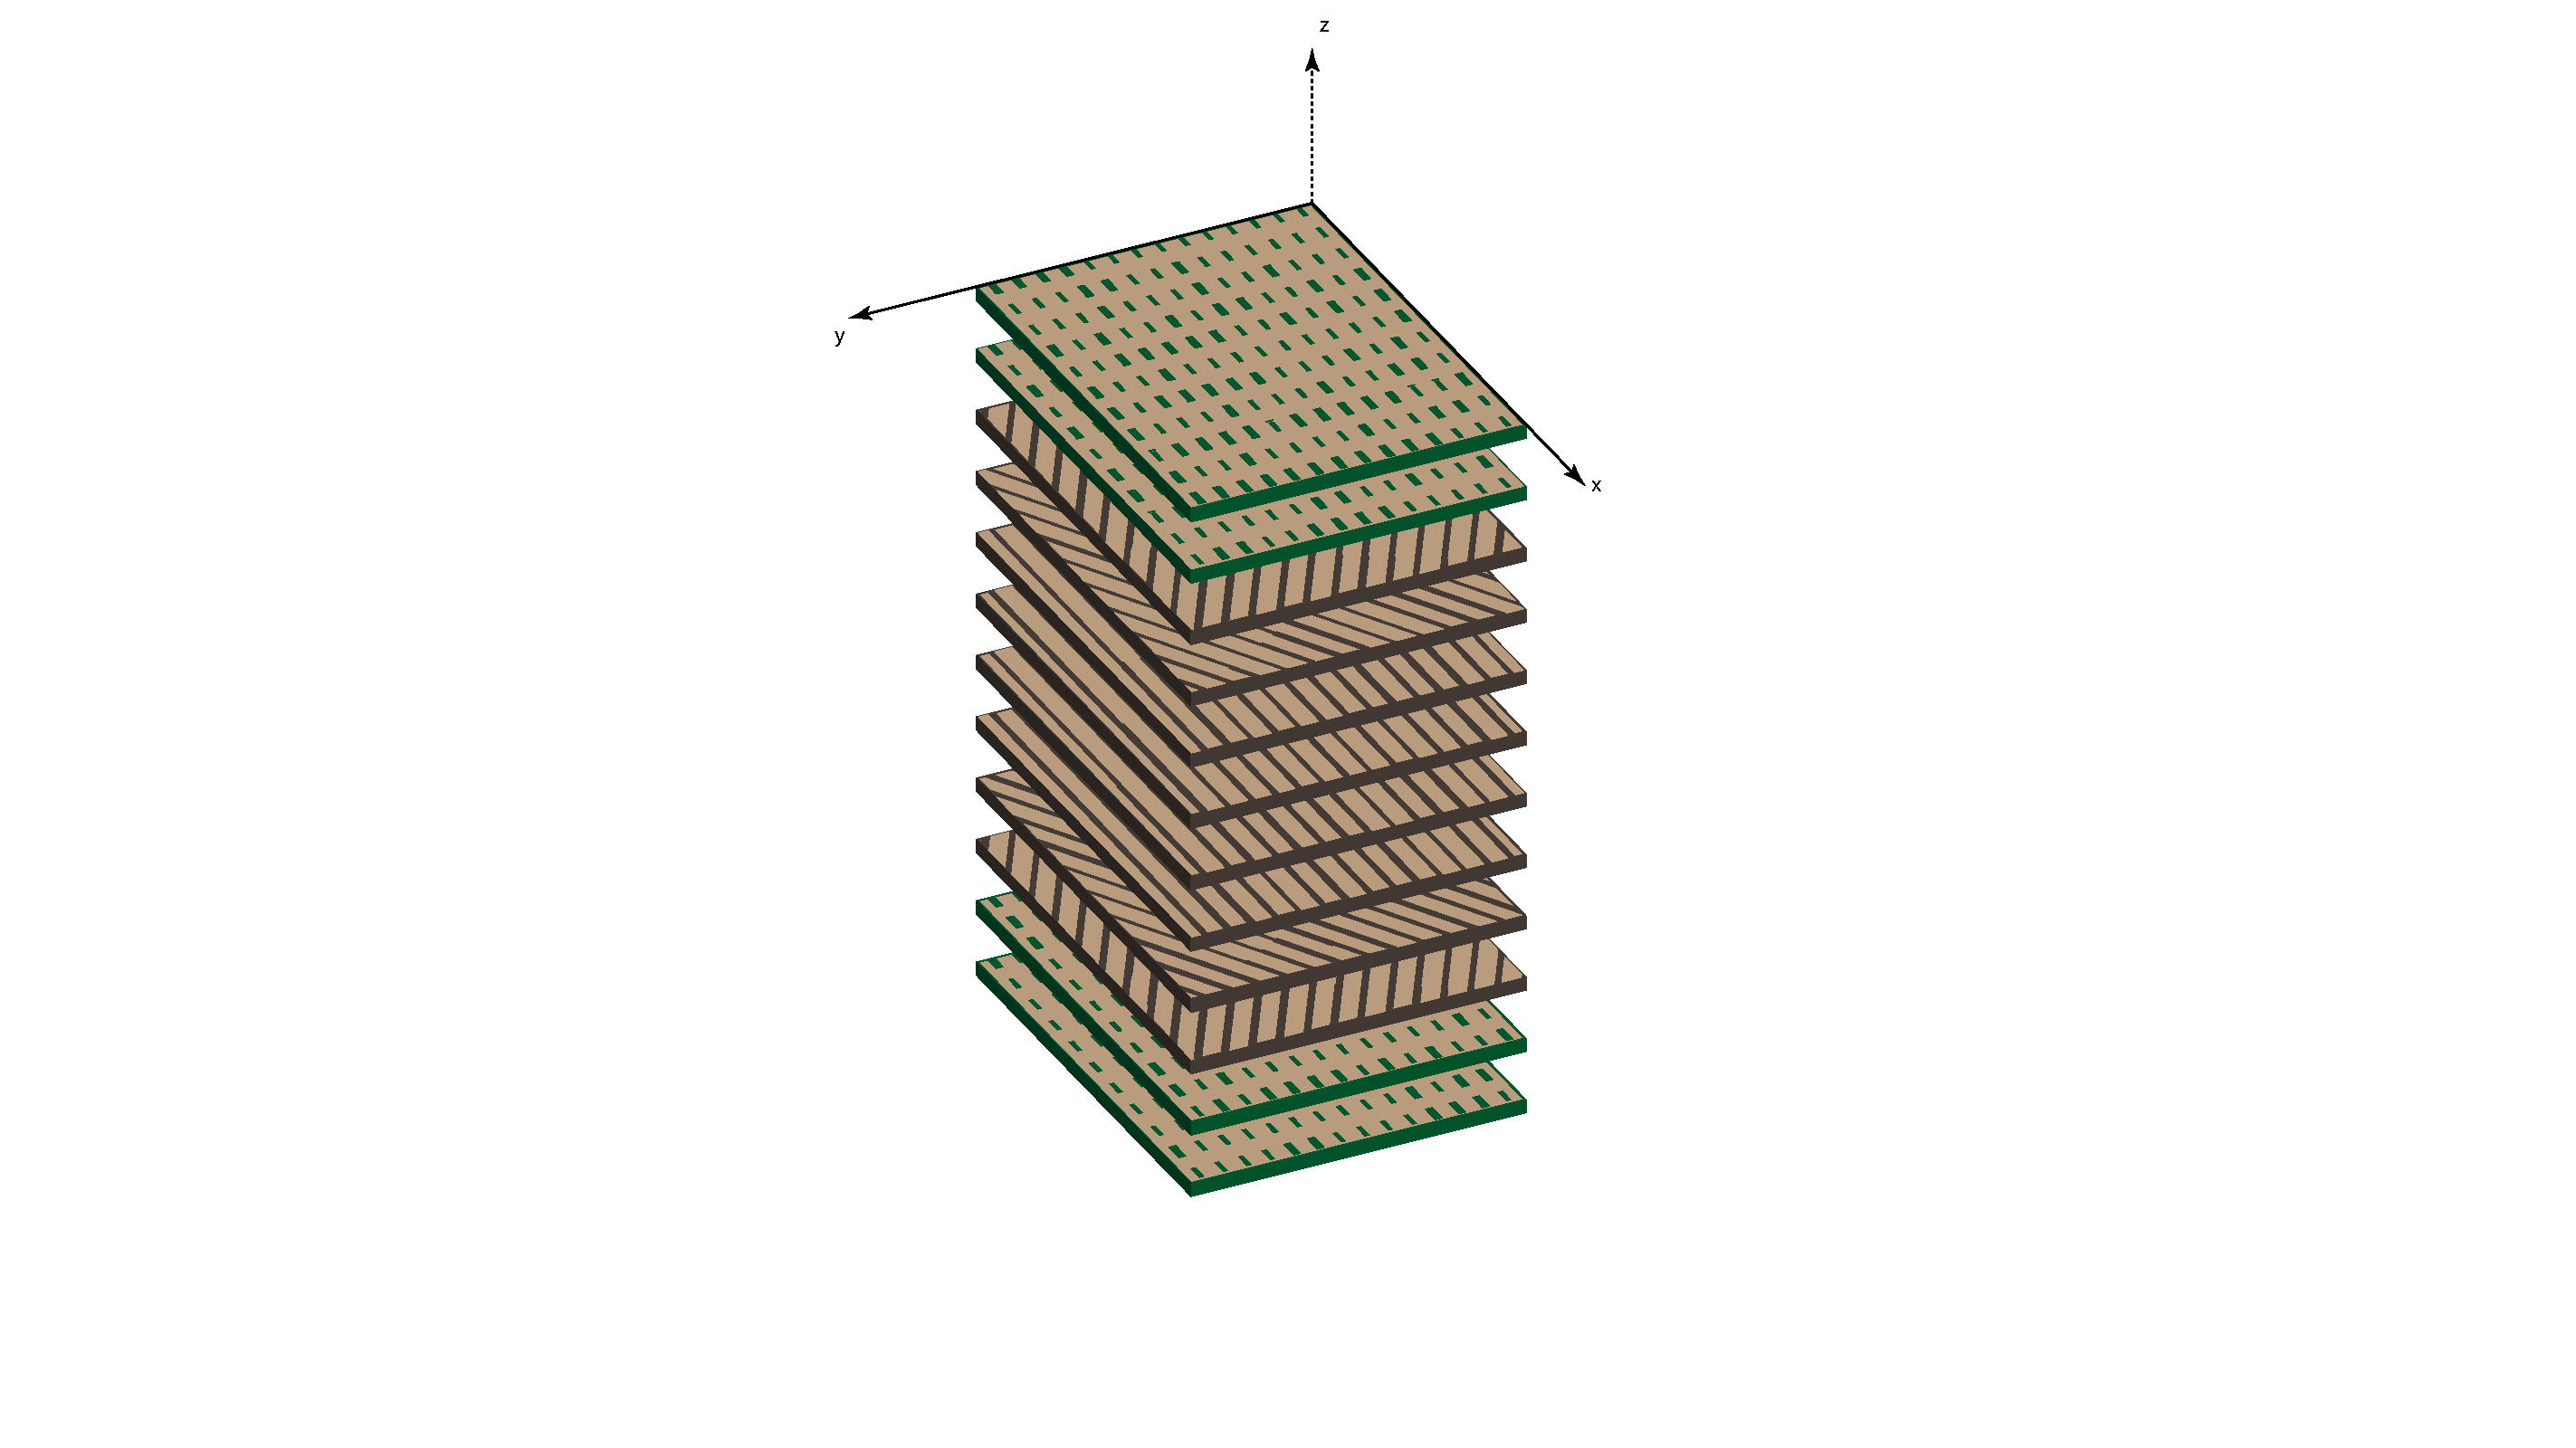
\includegraphics[width=\textwidth]{struct1.pdf}
		\caption{$[\alpha /-\alpha / 30 /-30 / 0_{2}]_{\mathrm{s}}$ }
		
	\end{subfigure}
	\hfill
	\begin{subfigure}[t]{0.24\textwidth}
		\centering
		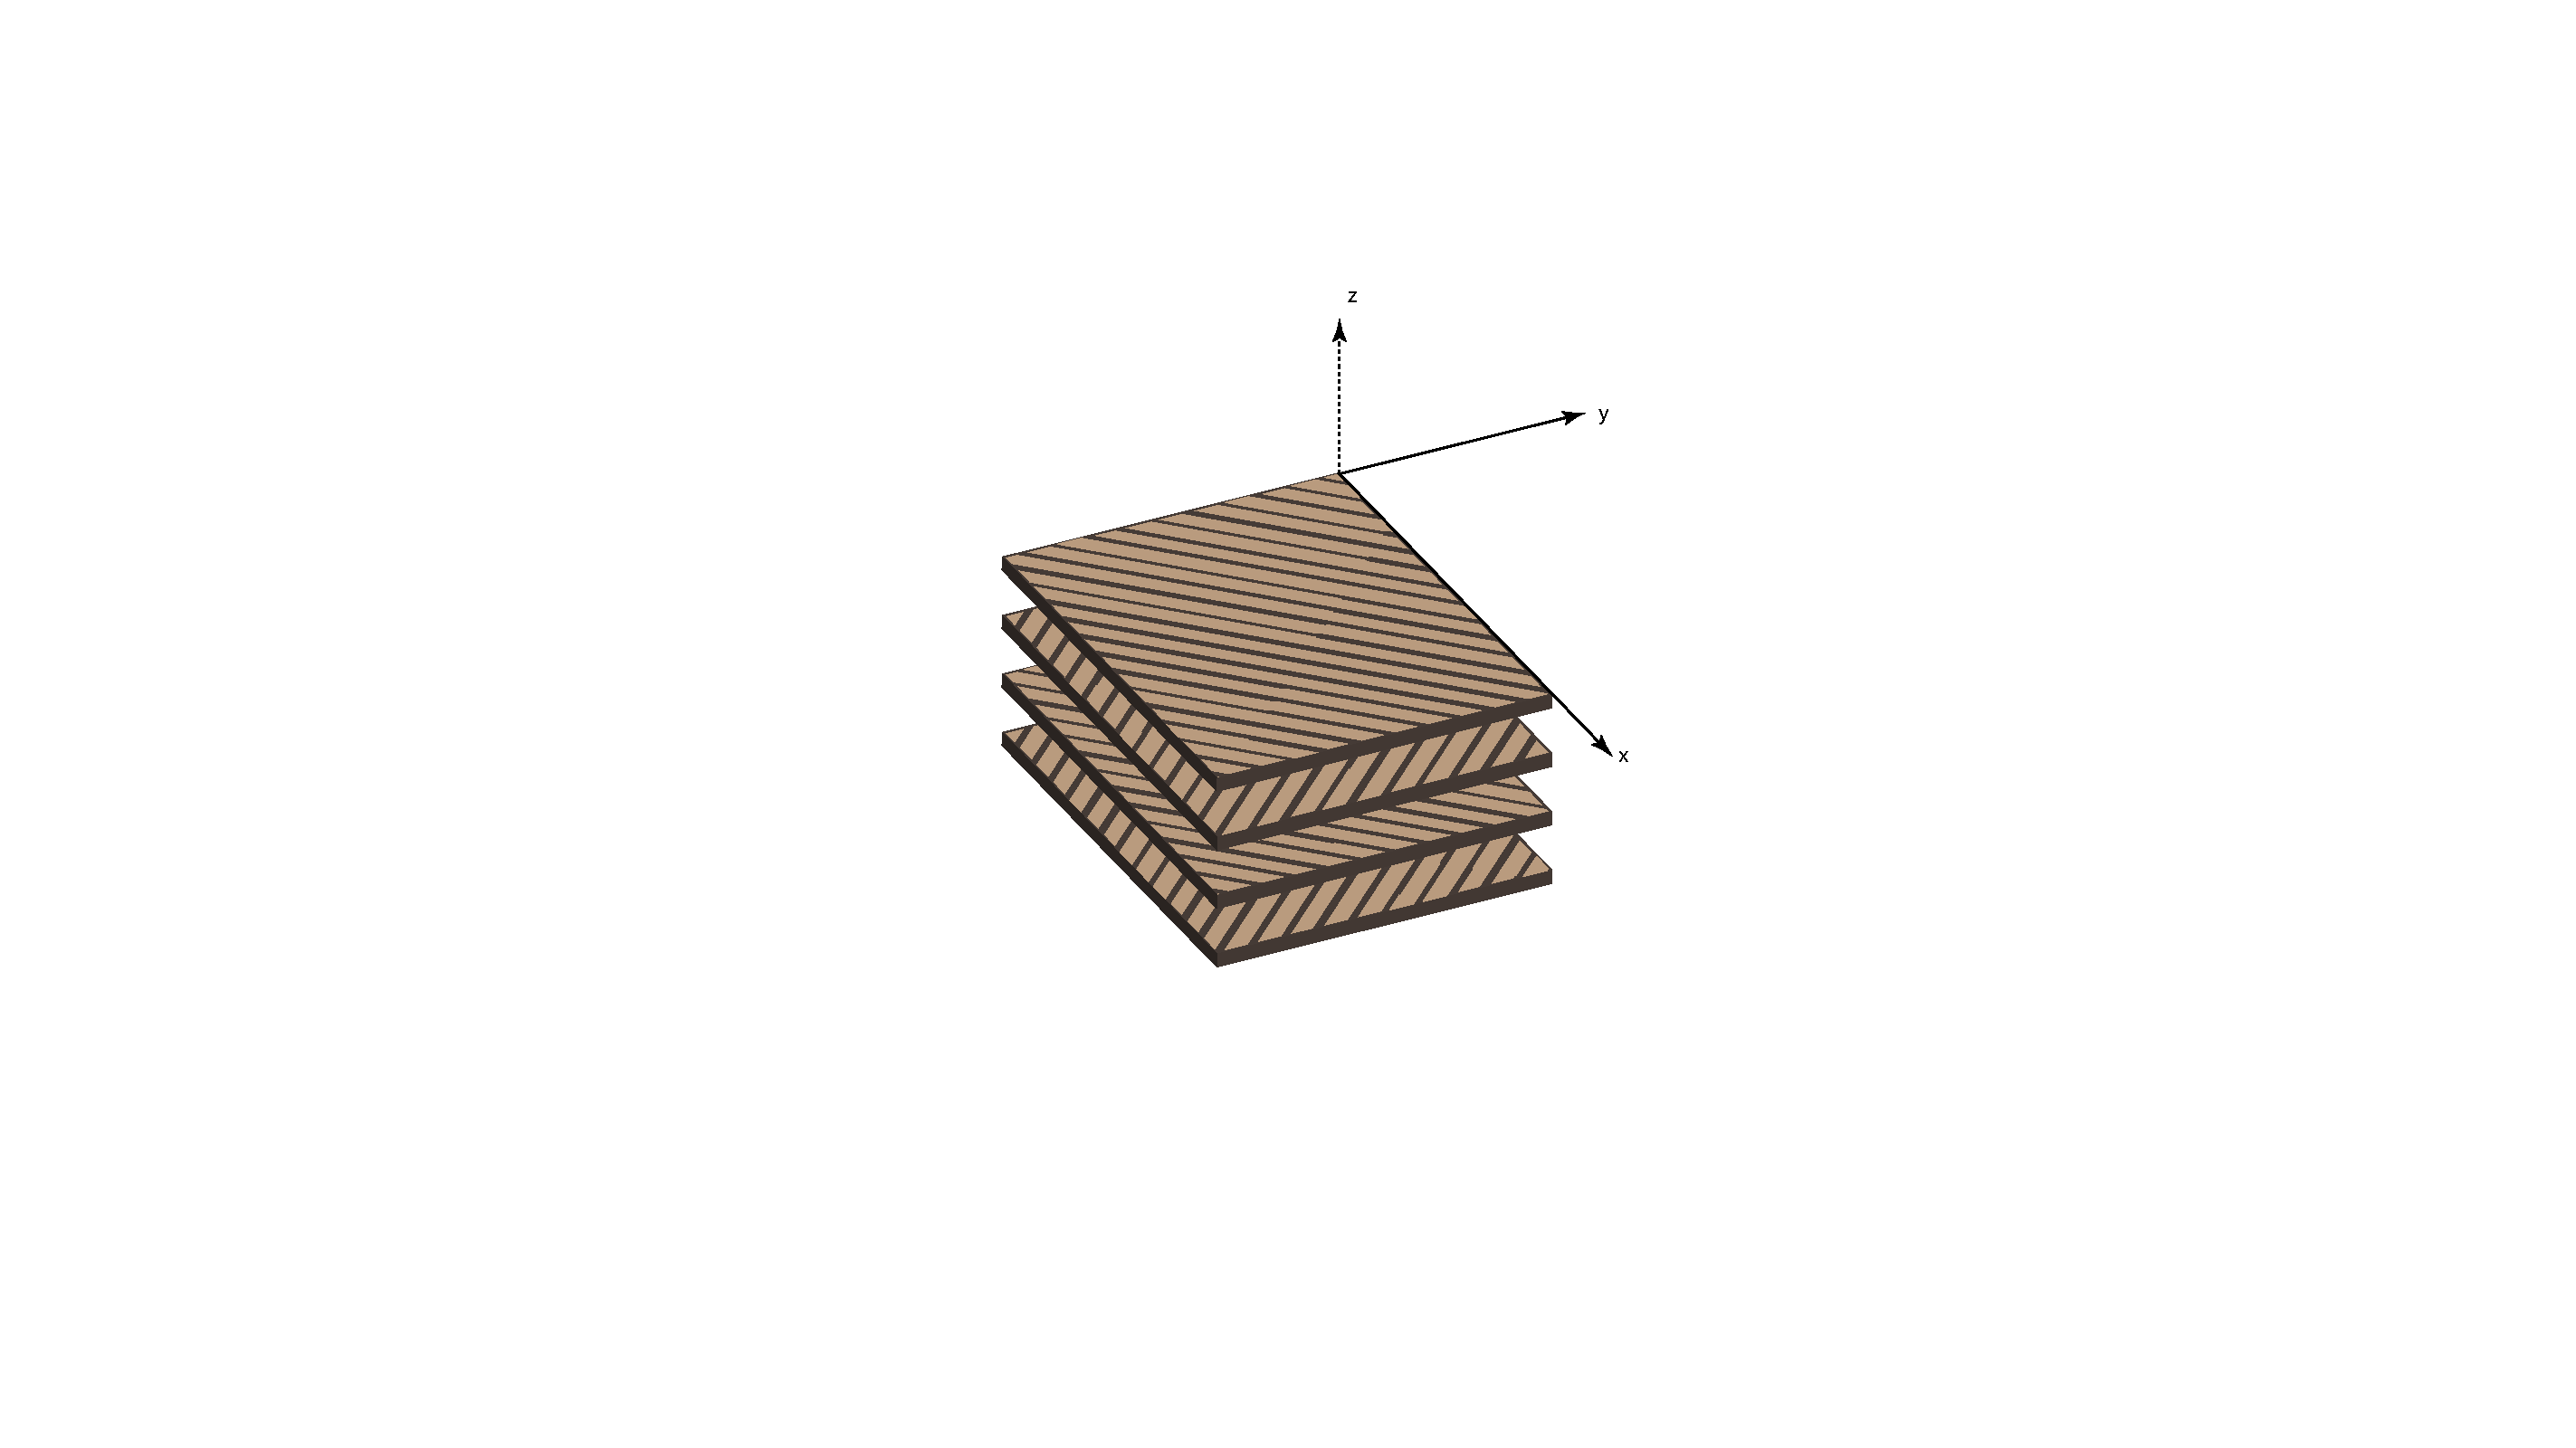
\includegraphics[width=\textwidth]{struct2.pdf}
		\caption{$[-45 / 45 /-45 / 45]$}
		
	\end{subfigure}
	\hfill
	\begin{subfigure}[t]{0.24\textwidth}
		\centering
		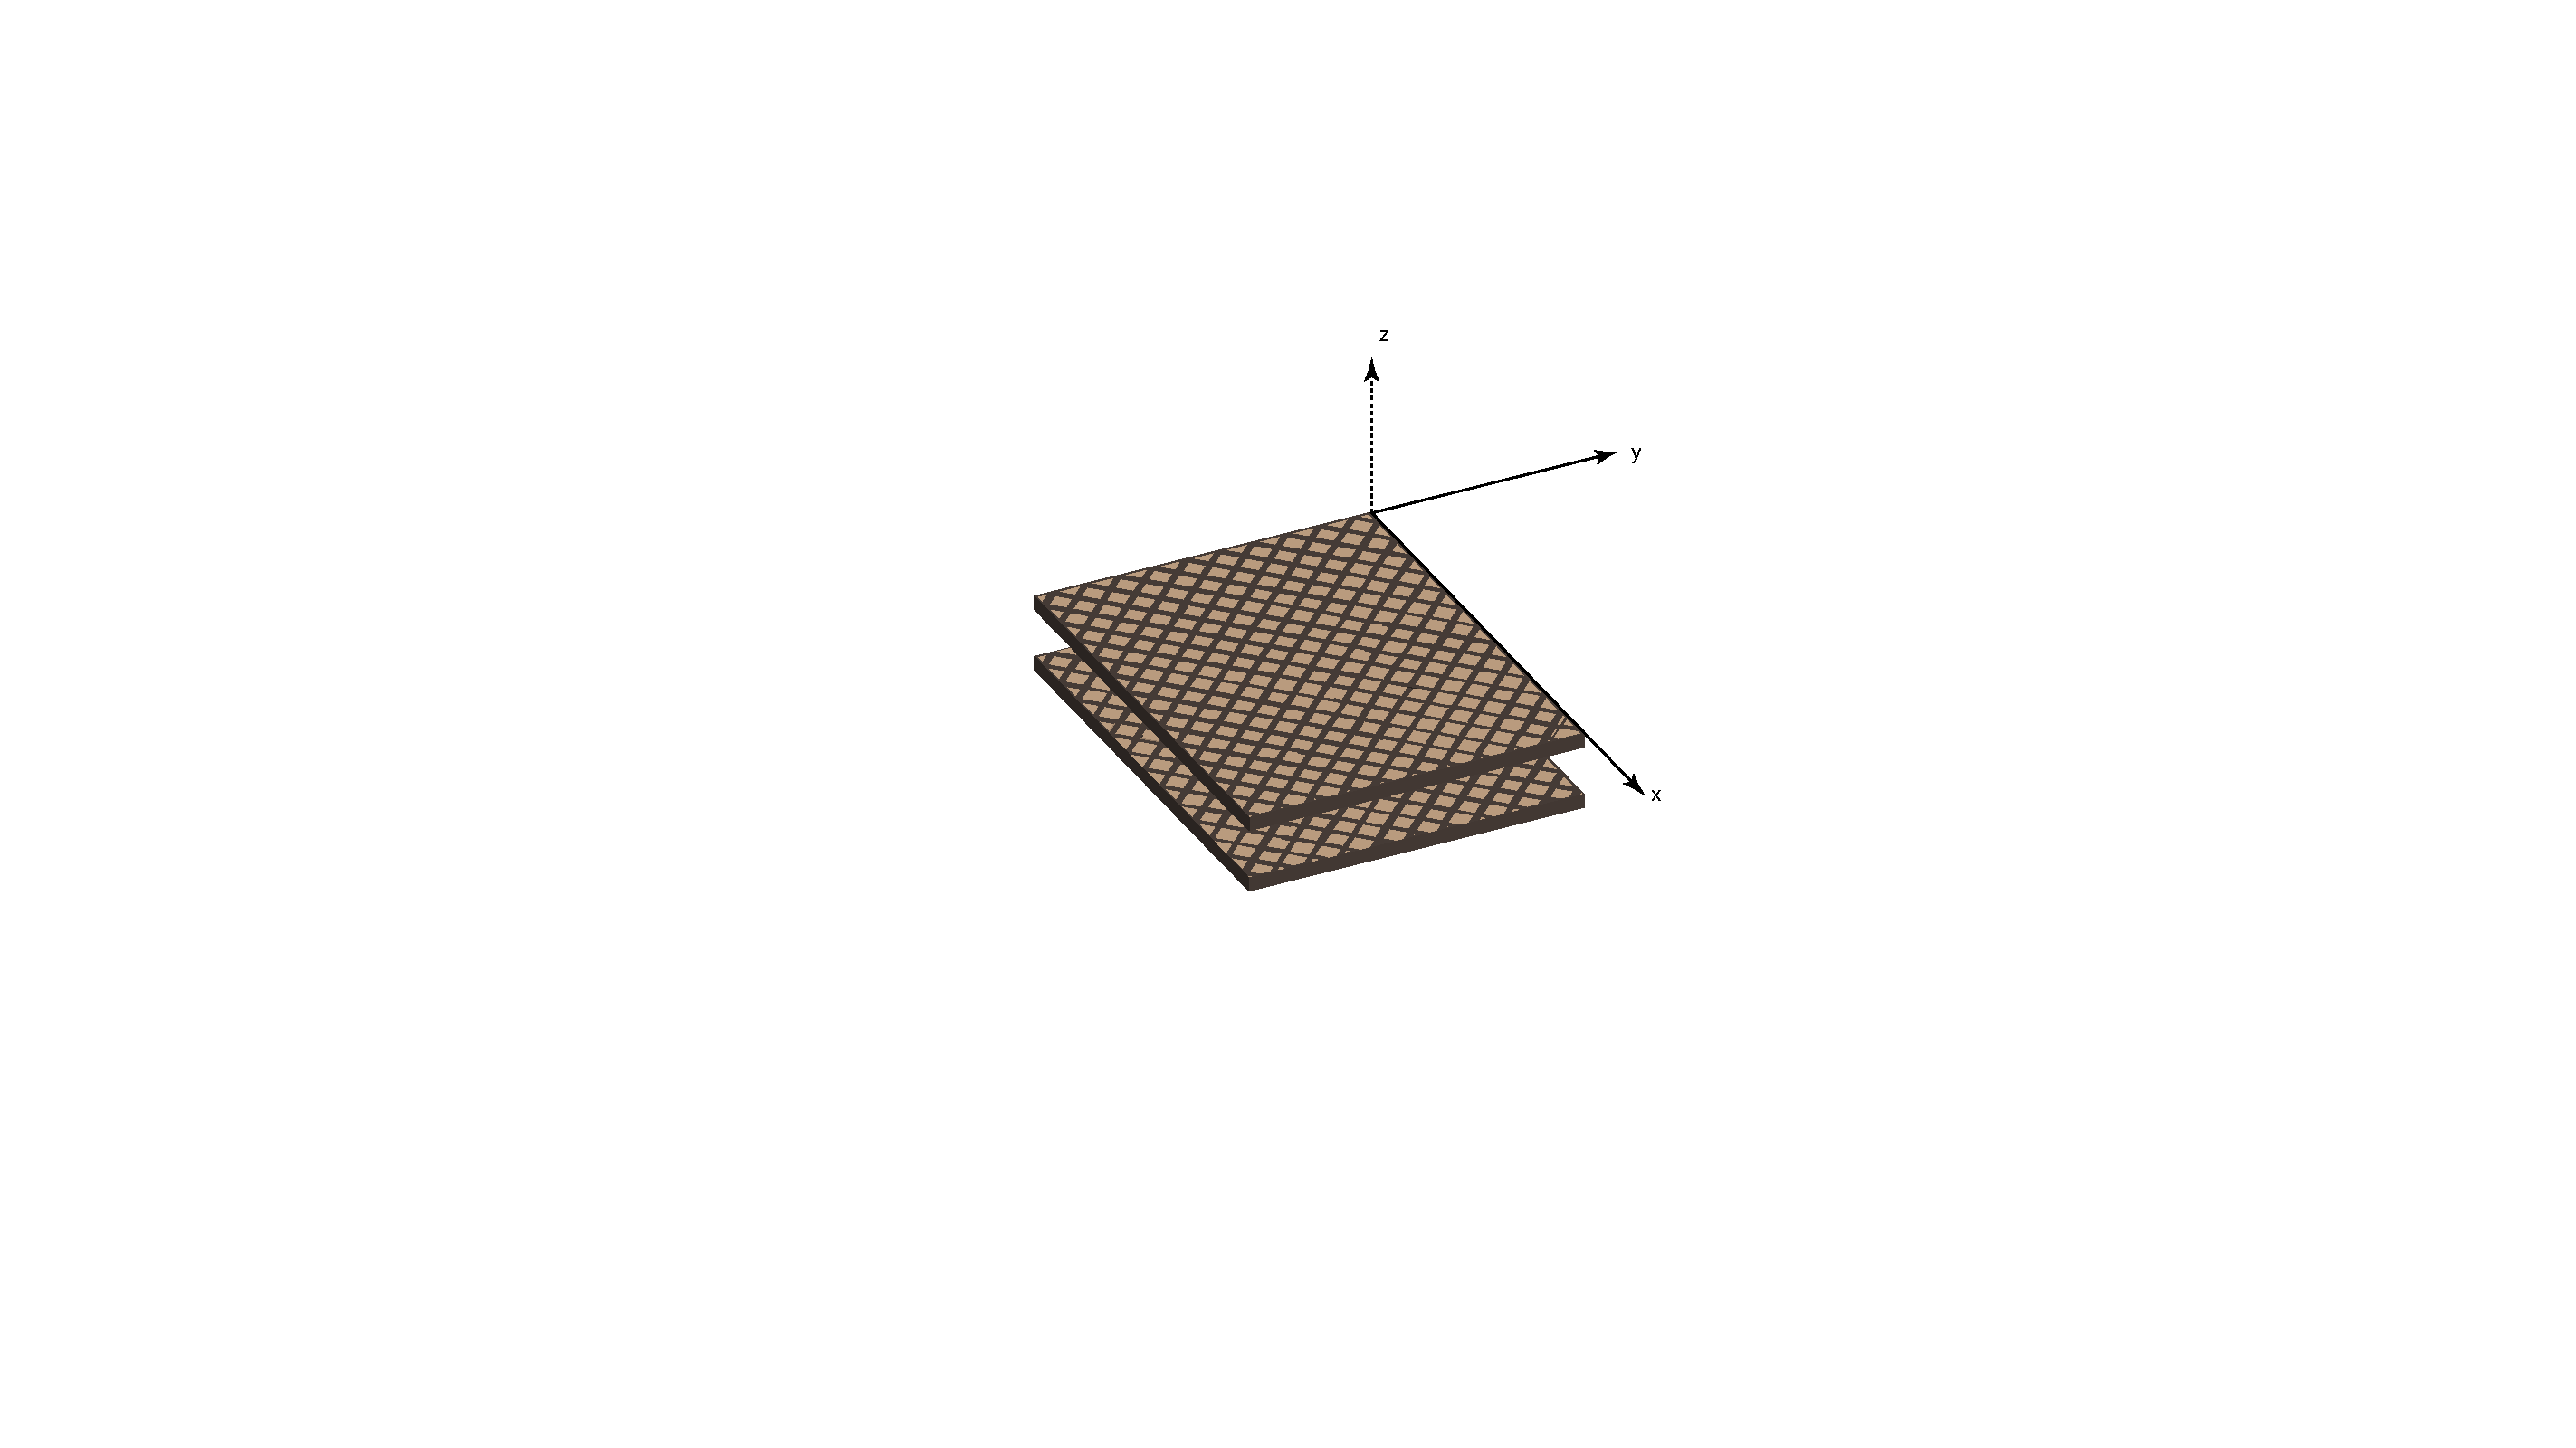
\includegraphics[width=\textwidth]{struct3.pdf}
		\caption{$[\pm 45^{f} / \pm 45^{f}]$}
		
	\end{subfigure}
	\hfill
	\begin{subfigure}[t]{0.24\textwidth}
		\centering
		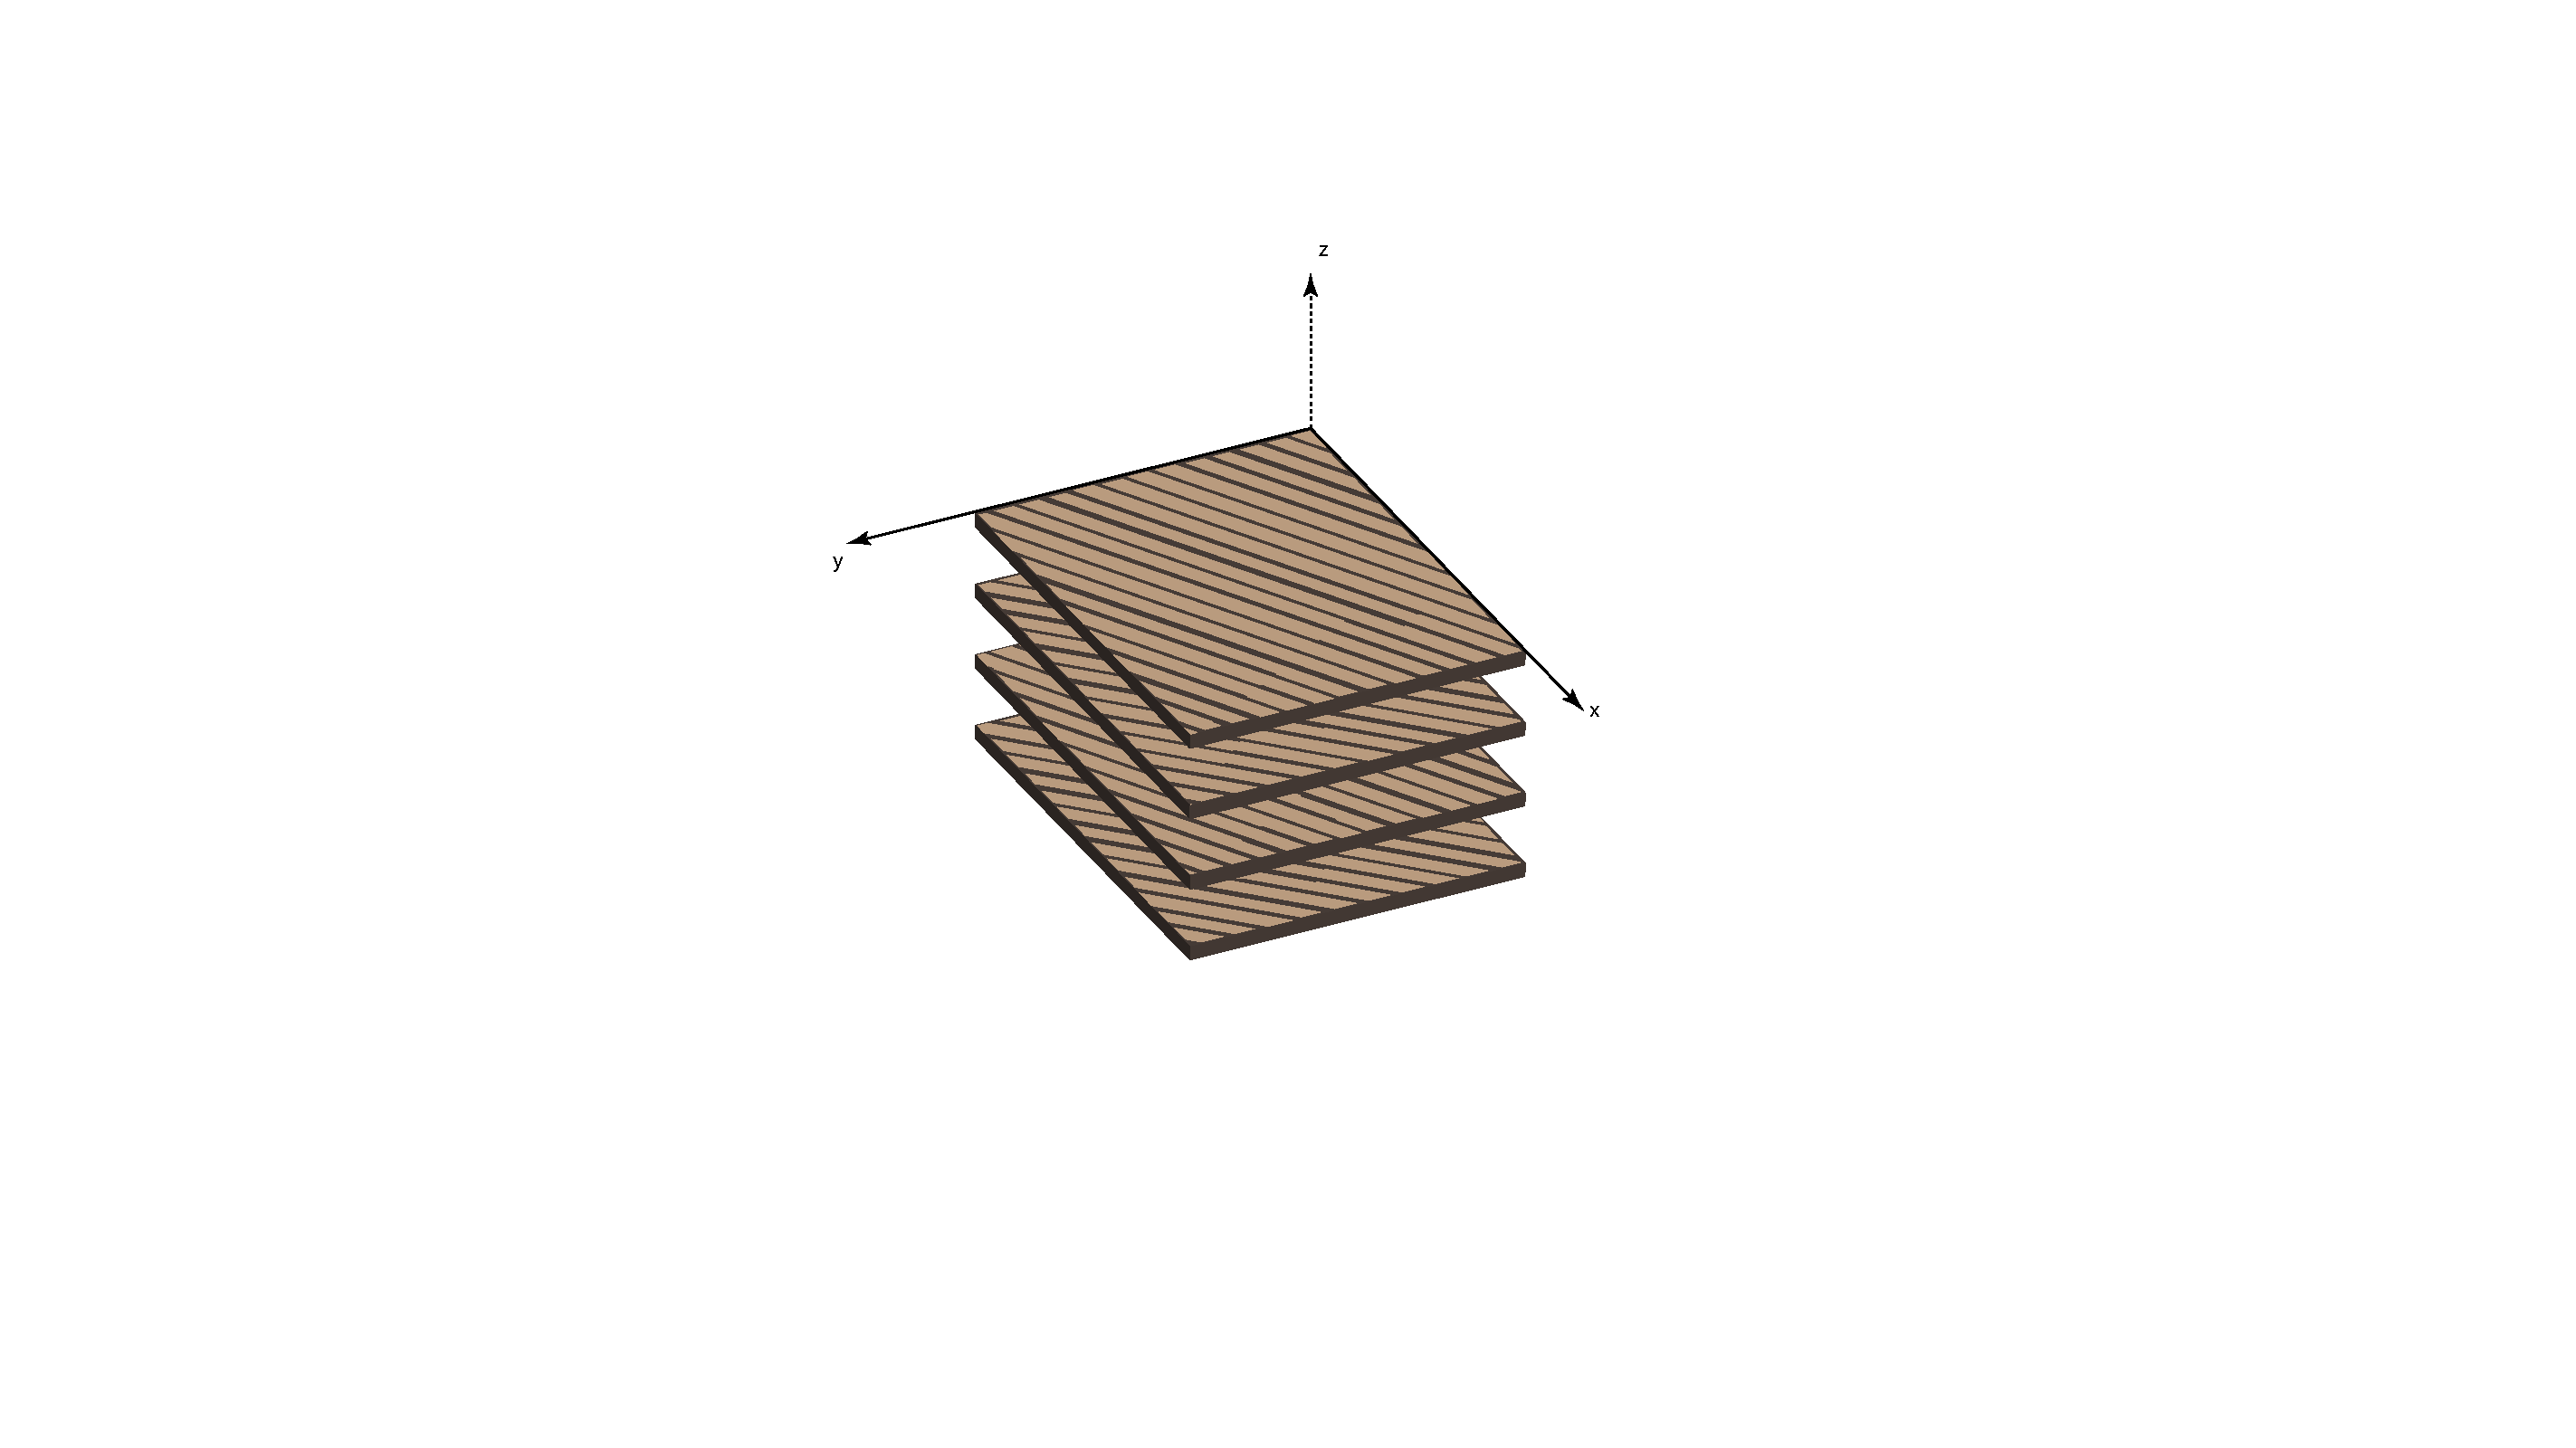
\includegraphics[width=\textwidth]{struct4.pdf}
		\caption{$[-30 /-45 /-30 /-45]$}
		
	\end{subfigure}
	\hfill
	\caption{Differenti layout di laminato }
	\label{fig:laminates}
\end{figure*}

Vengono affrontati 4 casi:

\begin{enumerate}[label=(\alph*)]
	\item $[\alpha /-\alpha / 30 /-30 / 0_{2}]_{\mathrm{s}}$ con $\alpha\in\left[0^\circ;90^\circ\right]$
	\item $[-45 / 45 /-45 / 45]$
	\item $[\pm 45^{f} / \pm 45^{f}]$
	\item $[-30 /-45 /-30 /-45]$
\end{enumerate}

Un'illustrazione rappresentativa dei differenti layout è presente in \cref{fig:laminates}.

Vengono affrontati anche due elementi strutturali differenti:
\begin{itemize}
\item Elemento tipo piastra
\item Elemento tipo cilindro
\end{itemize}

\begin{figure*}[bt!]
	\centering
	\begin{subfigure}[t]{0.24\textwidth}
		\centering

 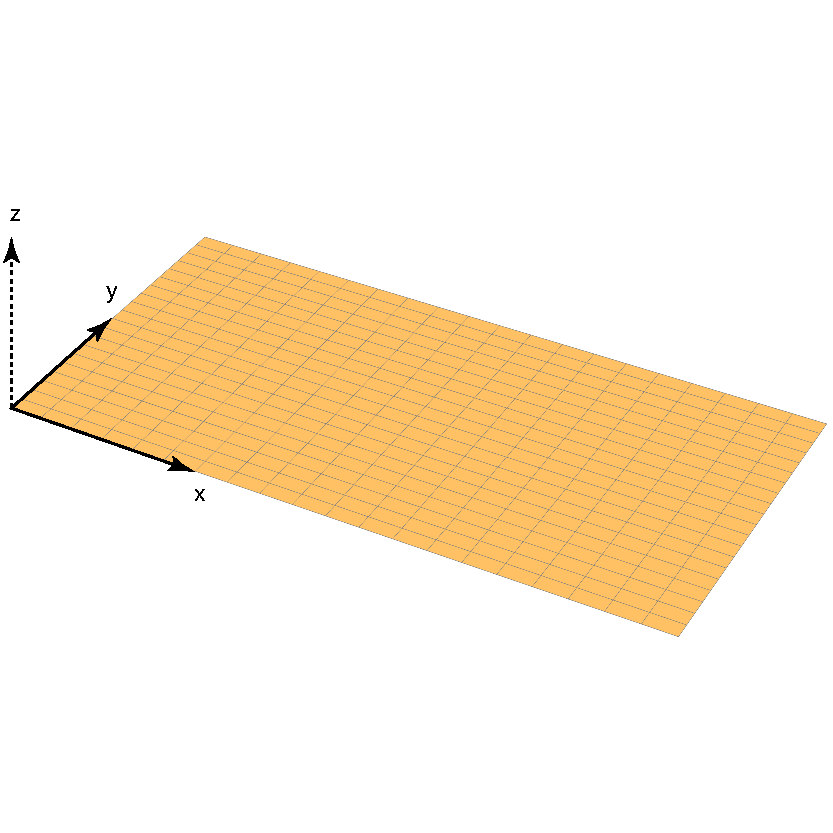
\includegraphics[width=\textwidth]{plate_.pdf}
 				\caption{Elemento tipo piastra}
		\label{fig:y equals x}
	\end{subfigure}
	\hfill
	\begin{subfigure}[t]{0.24\textwidth}
		\centering
		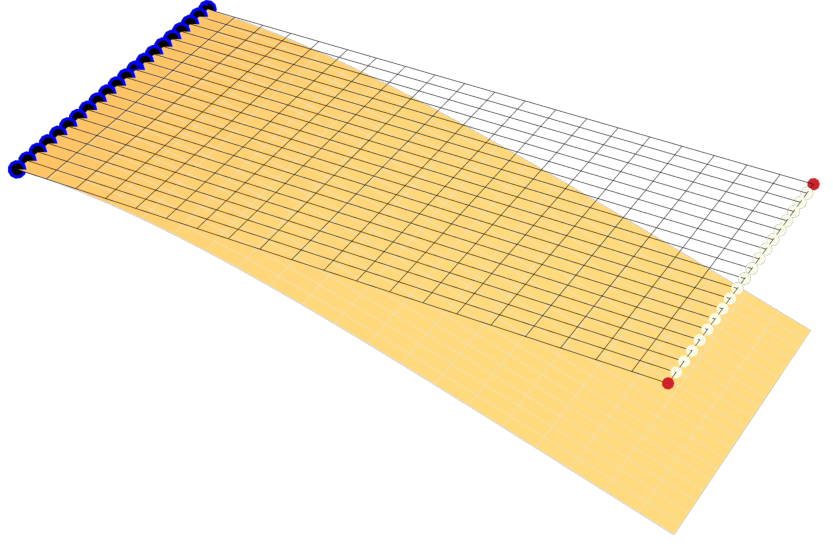
\includegraphics[width=\textwidth]{/first_test/alpha=40.pdf}
		\caption{Elemento tipo piastra deformato (caso \cref{sec:plate_A}  con $\alpha=40^\circ$ )}
		\label{fig:five over x}
	\end{subfigure}
	\hfill
	\begin{subfigure}[t]{0.24\textwidth}
		\centering
 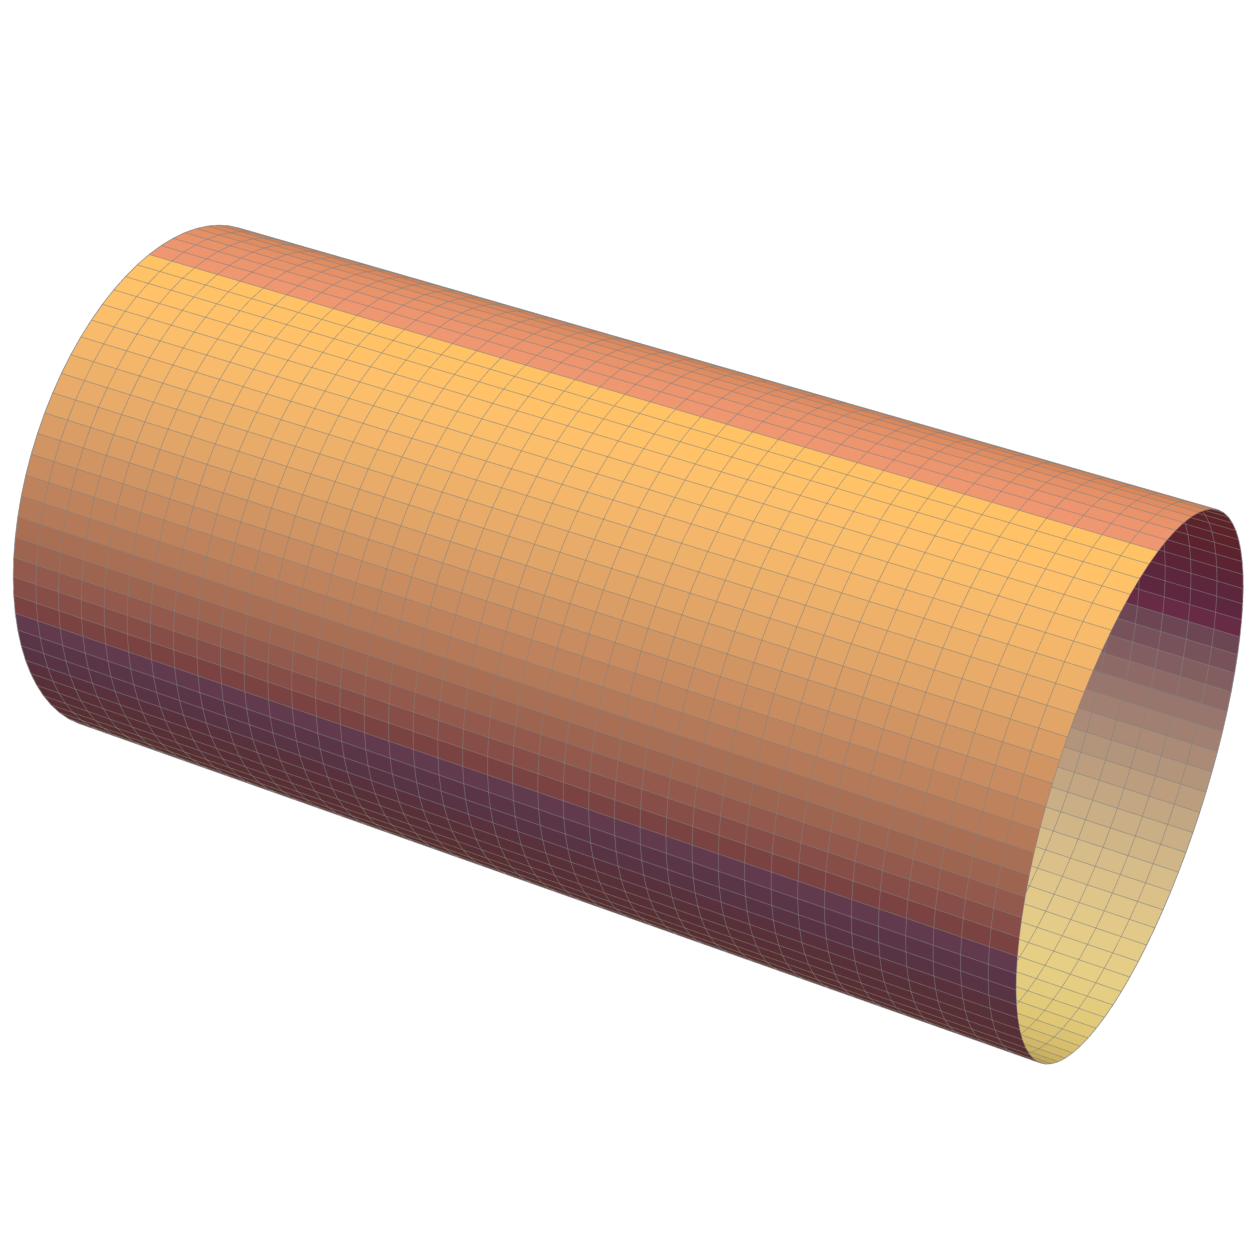
\includegraphics[width=\textwidth]{cyl_.pdf}
\caption{Elemento tipo cilindro}
		\label{fig:three sin x}
	\end{subfigure}
	\hfill
	\begin{subfigure}[t]{0.24\textwidth}
	\centering
 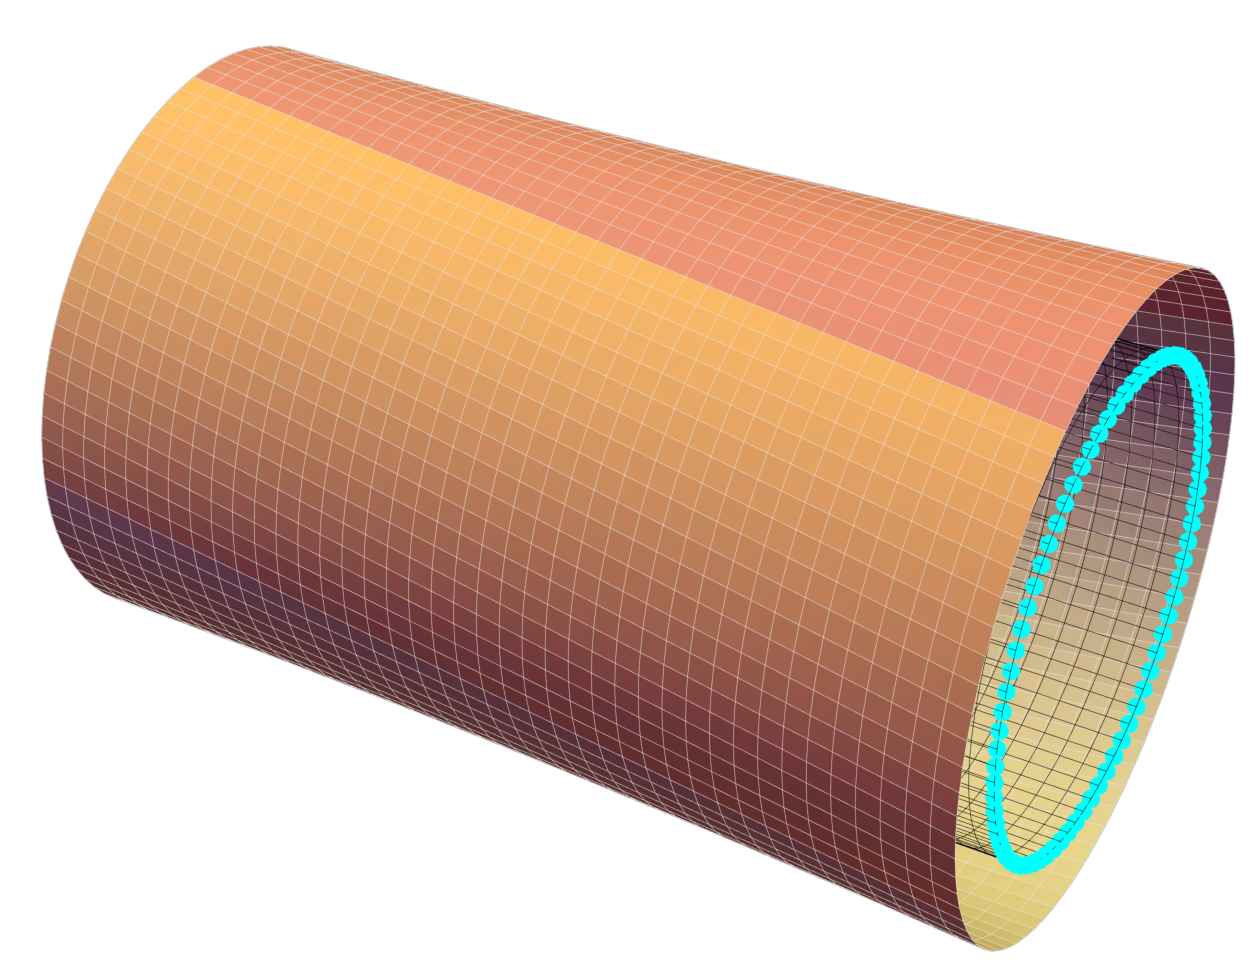
\includegraphics[width=\textwidth]{/more_test/cyl_30_45_30_45.pdf}
	\caption{Elemento tipo cilindro deformato (caso \cref{sec:cyl_C}}
	\label{fig:five ove x}
\end{subfigure}
	\hfill
	\caption{Elementi strutturali}
	\label{fig:three graphs}
\end{figure*}



COMPLETA CON ELENCO PUNTATO E DIFFERENTI CASI 

PRESENTA I DUE DIFFERENTI ELEEMTNI STRUTTURALI
\textcolor{blue}{\lipsum[1-2]}





\subsection{Elemento tipo piastra}
\subsubsection{Caso (a)}
\label{sec:plate_A}

\begin{figure*}[bt!]
	\centering

	\begin{subfigure}[t]{0.3\textwidth}
		\centering
		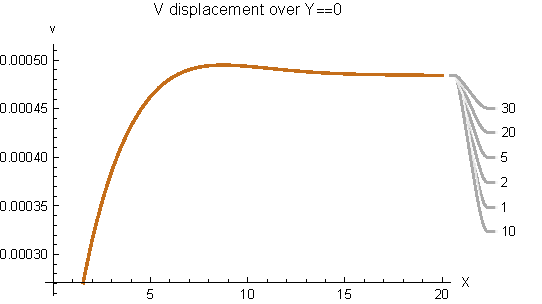
\includegraphics[width=\textwidth]{/first_test/bothload/V_X.pdf}
		\caption{Spostamento lungo $\hat y$ del bordo con $y=0$ della piastra}
		
	\end{subfigure}
	\hfill
	\begin{subfigure}[t]{0.3\textwidth}
		\centering
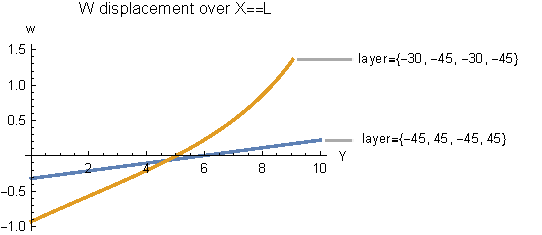
\includegraphics[width=\textwidth]{/first_test/bothload/W_Y.pdf}
		
		\caption{Effetto torsionale, spostamento lungo $\hat z$ del bordo estremale della piastra ($x=L$)}
		
	\end{subfigure}
	\hfill
	\begin{subfigure}[t]{0.3\textwidth}
		\centering
		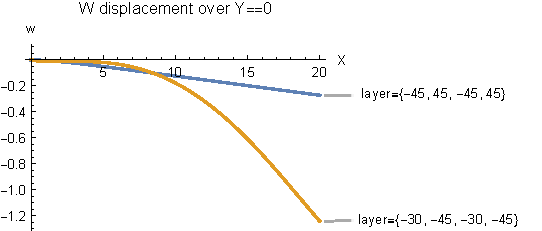
\includegraphics[width=\textwidth]{/first_test/bothload/W_X.pdf}
		\caption{Effetto flessionale, spostamento lungo $z$ del bordo $y=0$ della piastra}
		
	\end{subfigure}
	\hfill
	\caption{Risultati caso (a) per un elemento strutturale tipo piastra con entrambi i carichi (\cref{sec:plate_A})}
	\label{fig:plate_A_both_load}
\end{figure*}


\begin{figure*}[bt!]
	\centering
	
	\begin{subfigure}[t]{0.3\textwidth}
		\centering
		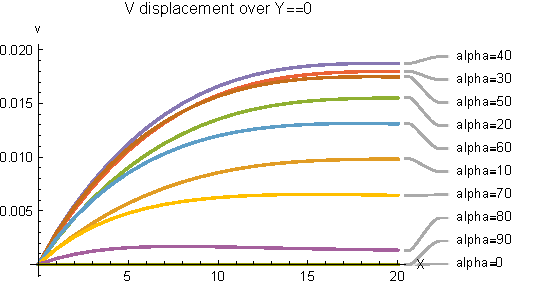
\includegraphics[width=\textwidth]{/first_test/transversal_load/V_X.pdf}
		\caption{Spostamento lungo $\hat y$ del bordo con $y=0$ della piastra}
		
	\end{subfigure}
	\hfill
	\begin{subfigure}[t]{0.3\textwidth}
		\centering
		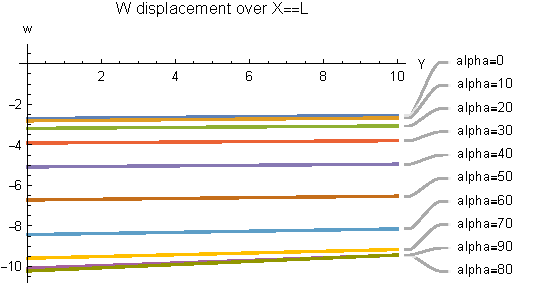
\includegraphics[width=\textwidth]{/first_test/transversal_load/W_Y.pdf}
		
		\caption{Effetto torsionale, spostamento lungo $\hat z$ del bordo estremale della piastra ($x=L$)}
		
	\end{subfigure}
	\hfill
	\begin{subfigure}[t]{0.3\textwidth}
		\centering
		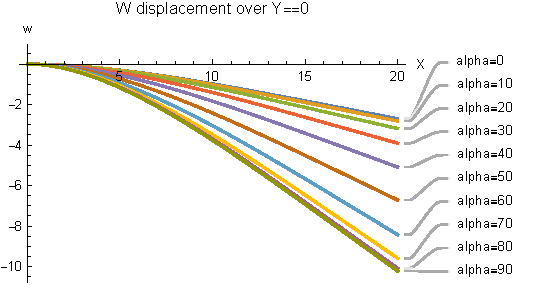
\includegraphics[width=\textwidth]{/first_test/transversal_load/W_X.pdf}
		\caption{Effetto flessionale, spostamento lungo $z$ del bordo $y=0$ della piastra}
		
	\end{subfigure}
	\hfill
	\caption{Risultati caso (a) per un elemento strutturale tipo piastra con carichi tipo trasversale (\cref{sec:plate_A})}
	\label{fig:plate_A_transload_load}
\end{figure*}

\begin{figure*}[bt!]
	\centering
	
	\begin{subfigure}[t]{0.3\textwidth}
		\centering
		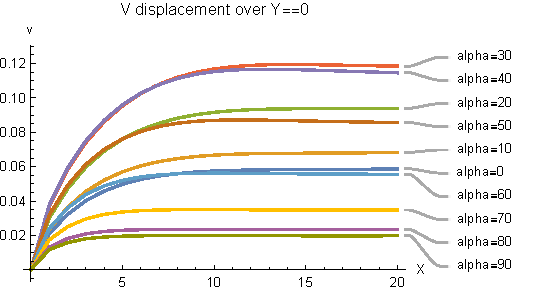
\includegraphics[width=\textwidth]{/first_test/axial_load/V_X.pdf}
		\caption{Spostamento lungo $\hat y$ del bordo con $y=0$ della piastra}
		
	\end{subfigure}
	\hfill
	\begin{subfigure}[t]{0.3\textwidth}
		\centering
		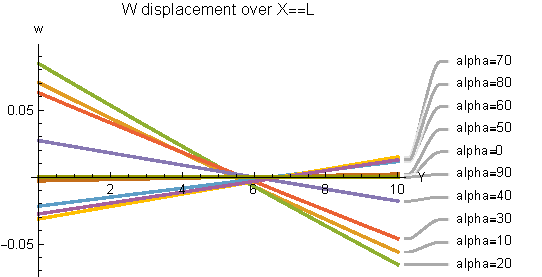
\includegraphics[width=\textwidth]{/first_test/axial_load/W_Y.pdf}
		
		\caption{Effetto torsionale, spostamento lungo $\hat z$ del bordo estremale della piastra ($x=L$)}
		
	\end{subfigure}
	\hfill
	\begin{subfigure}[t]{0.3\textwidth}
		\centering
		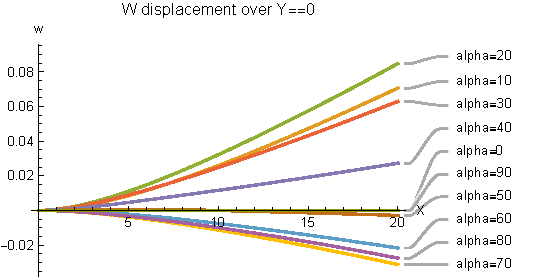
\includegraphics[width=\textwidth]{/first_test/axial_load/W_X.pdf}
		\caption{Effetto flessionale, spostamento lungo $z$ del bordo $y=0$ della piastra}
		
	\end{subfigure}
	\hfill
	\caption{Risultati caso (a) per un elemento strutturale tipo piastra con carichi tipo assiale(\cref{sec:plate_A})}
	\label{fig:plate_A_axial_load}
\end{figure*}


\textcolor{blue}{\lipsum[1-2]}


\subsubsection{Caso (b)}
\textcolor{blue}{\lipsum[1-2]}
\subsubsection{Caso (c)}
\textcolor{blue}{\lipsum[1-2]}
\subsubsection{Caso (d)}
\textcolor{blue}{\lipsum[1-2]}

\subsection{Elemento tipo cilindro}

\subsubsection{Caso (a)}
\textcolor{blue}{\lipsum[1-2]}
\subsubsection{Caso (b)}
\label{sec:cyl_B}
\textcolor{blue}{\lipsum[1-2]}
\subsubsection{Caso (c)}
\label{sec:cyl_C}
\textcolor{blue}{\lipsum[1-2]}
\subsubsection{Caso (d)}
\textcolor{blue}{\lipsum[1-2]}


\section{Spessore della piastra}

Consideriamo un ulteriore caso con un layout $[10 /-10 / 30 /-30 / 0_2]_{\mathrm{s}}$ illustrato in \cref{fig:last_case_schema}. 

\begin{figure*}[bt!]
	\centering
	\begin{subfigure}[t]{0.3\textwidth}
		\centering
		
		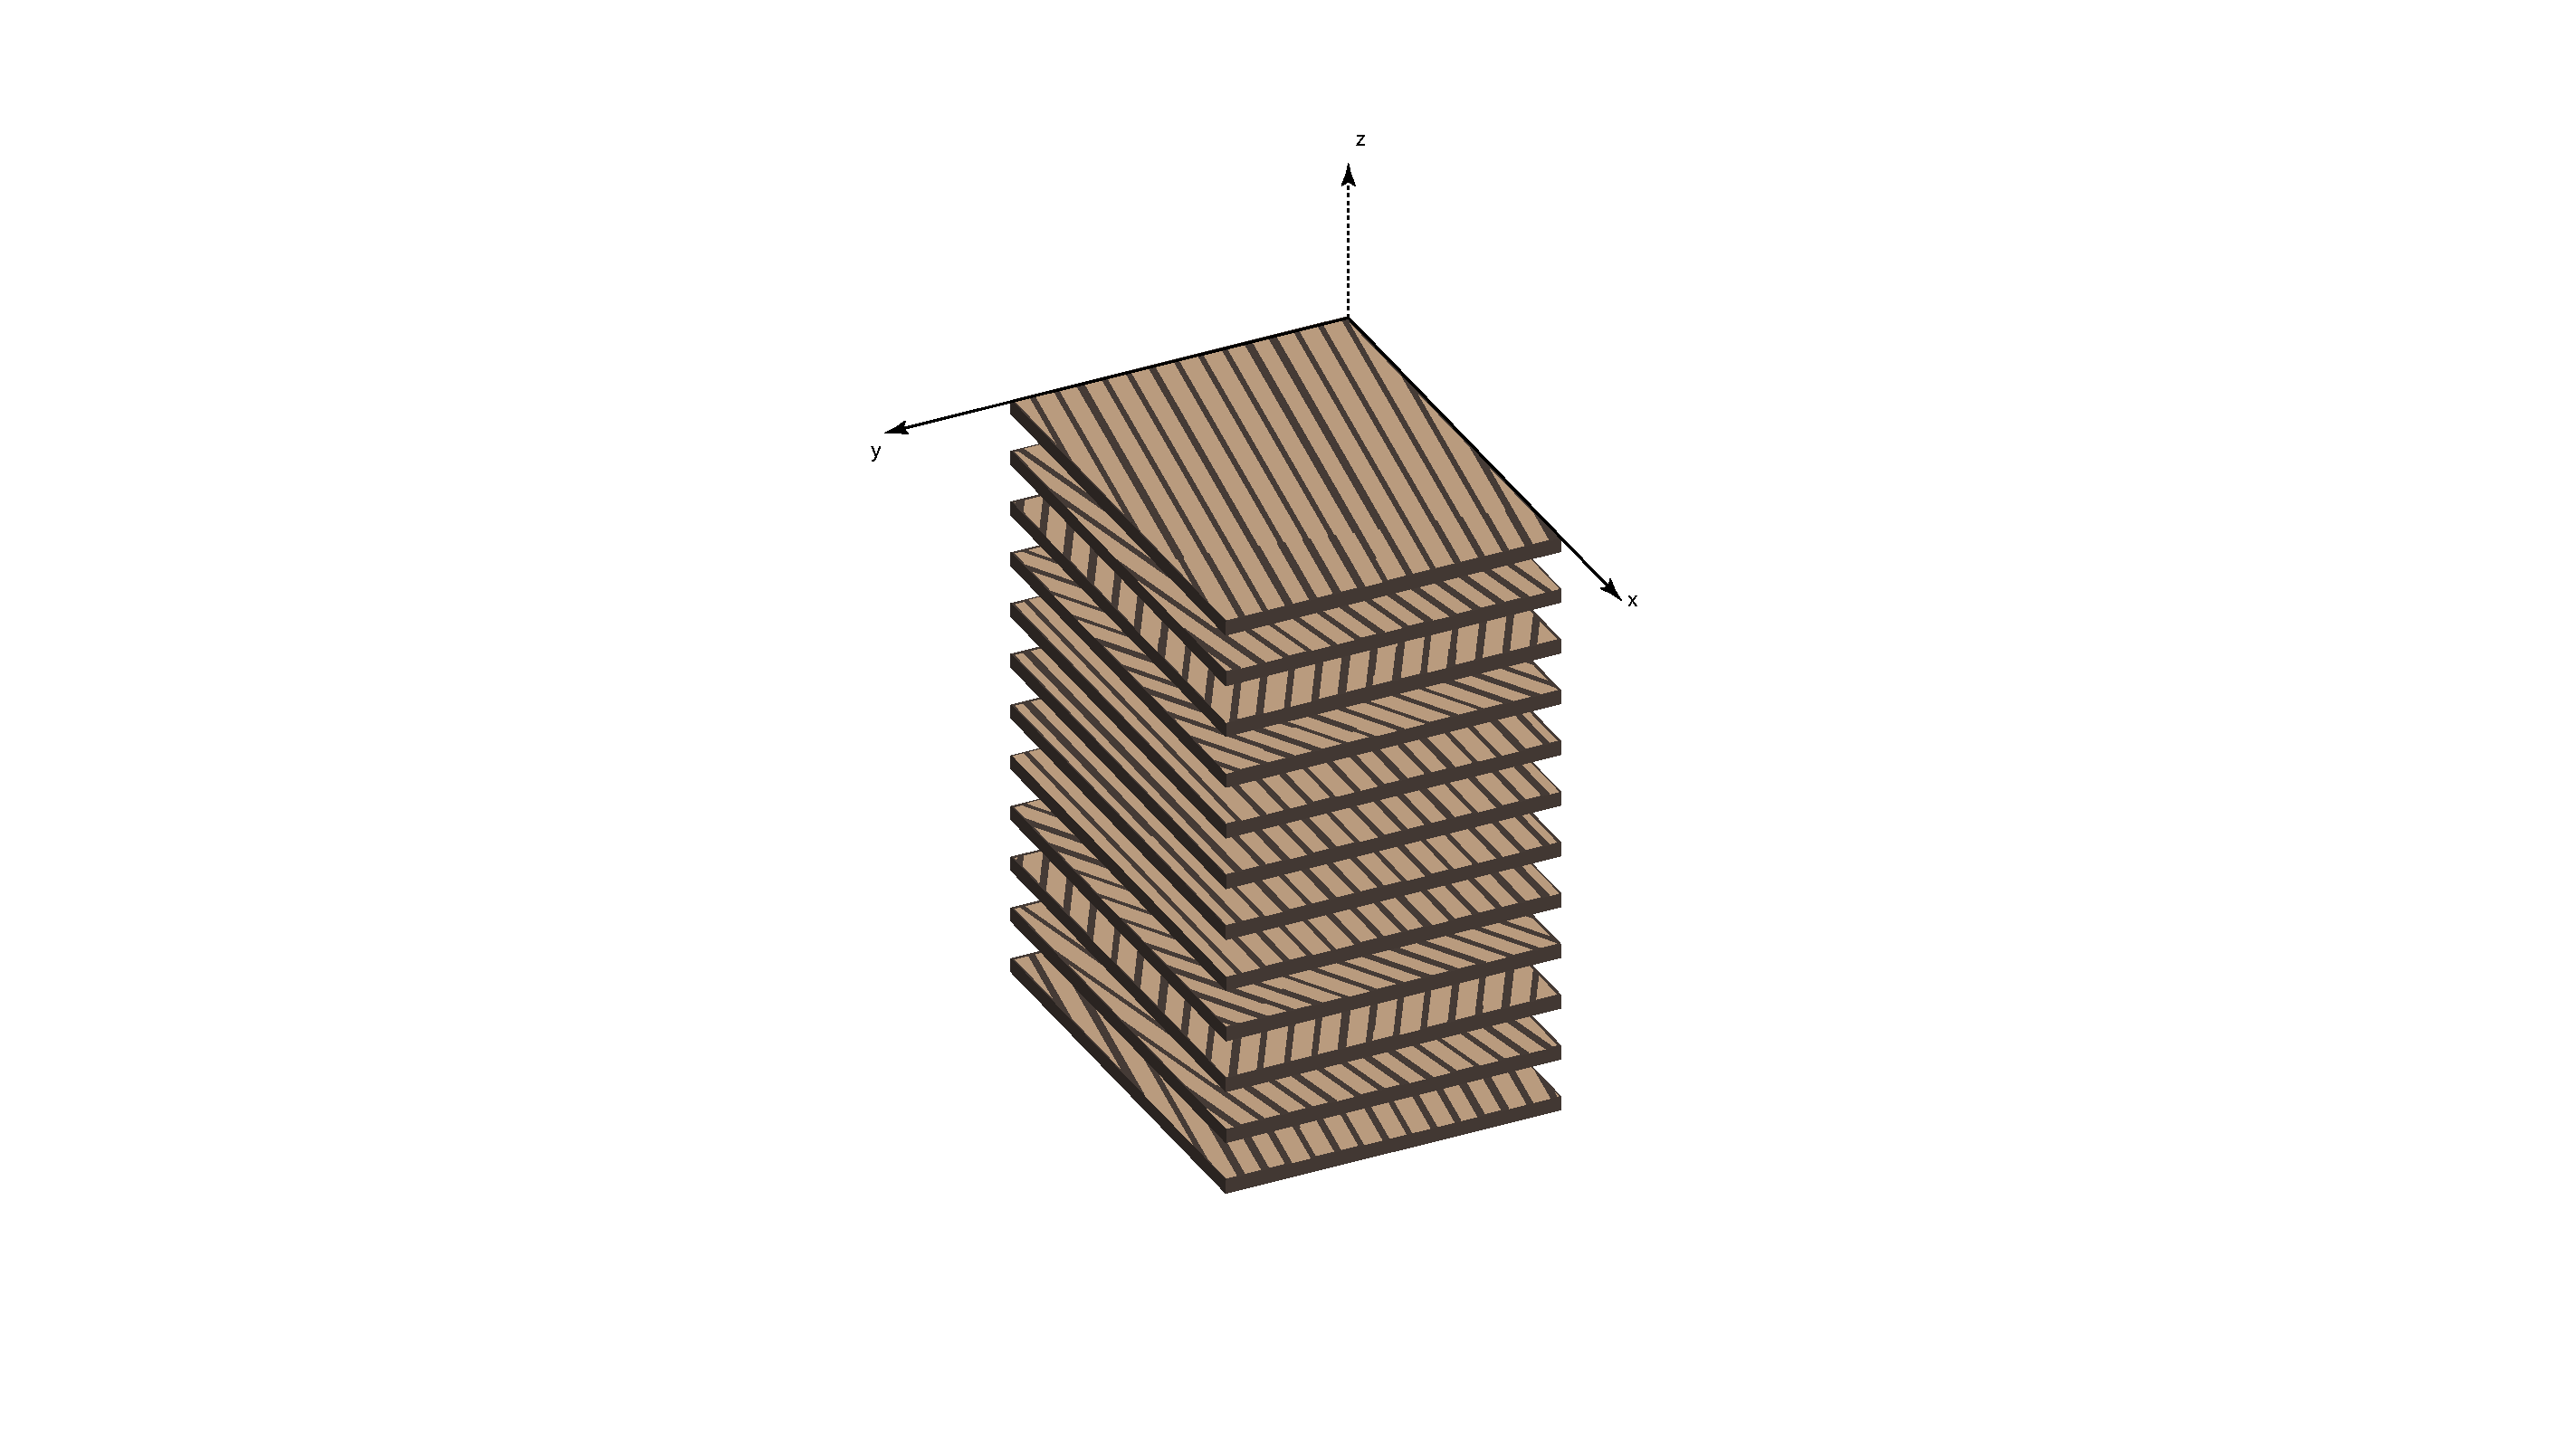
\includegraphics[width=\textwidth]{struct5.pdf}
		\caption{Descrizione}
			\label{fig:last_case_schema}
	\end{subfigure}
	\hfill
	\begin{subfigure}[t]{0.3\textwidth}
		\centering
		METTI FIGURA DI PROFILO CON RETTANGOLI CON GRADI
		%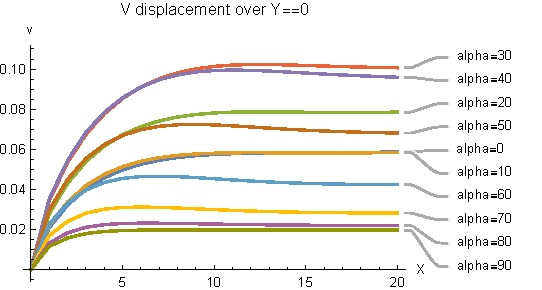
\includegraphics[width=\textwidth]{V_X=.pdf}
		\caption{Descrizione}
		
	\end{subfigure}
	\hfill
	\begin{subfigure}[t]{0.3\textwidth}
		\centering
		%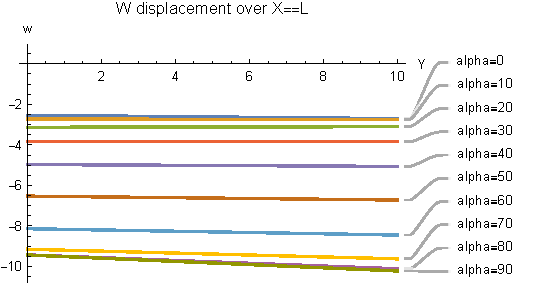
\includegraphics[width=\textwidth]{W_Y=.pdf}
		\caption{Descrizione}
		
	\end{subfigure}
	\hfill
	\caption{ DESCRIZIONE }
	\label{fig:last_case}
\end{figure*}

\textcolor{blue}{\lipsum[1-2]}


\section{Conclusioni}

\textcolor{blue}{\lipsum[1-2]}
\section{Metodi}

\textcolor{blue}{\lipsum[1-2]}


\section{Disponibilità del codice e materiale aggiuntivo}

Tutto il codice, le immagini, file di processamento e risultati ottenuti sono disponibili alla repository online al link: \url{https://github.com/mastroalex/comp-lam}. 

Il codice 


\subsection{Lista delle abbreviazioni}

\begin{itemize}
	\item CF, carbon fiber
\end{itemize}
 


%% Specify your .bib file name here, without the extension
%\newpage
%\onecolumn

\newpage
\bibliography{paper-refs}




\end{document}
